\documentclass[10pt,compress,xcolor={dvipsnames,usennames,table}]{beamer}

\usetheme{Frankfurt}
% other themes: AnnArbor, Antibes, Bergen, Berkeley, Berlin, Boadilla, boxes, CambridgeUS, Copenhagen, Darmstadt, default, Dresden, Frankfurt, Goettingen,
% Hannover, Ilmenau, JuanLesPins, Luebeck, Madrid, Maloe, Marburg, Montpellier, PaloAlto, Pittsburg, Rochester, Singapore, Szeged, classic

% \usecolortheme{whale}
\definecolor{db}{rgb}{0.45, 0.0, 0.4}
\usecolortheme[named=db]{structure} 
% color themes: albatross, beaver, beetle, crane, default, dolphin, dov, fly, lily, orchid, rose, seagull, seahorse, sidebartab, structure, whale, wolverine

\usepackage[utf8]{inputenc}
\usepackage[spanish]{babel}
\usepackage{amsmath}
\usepackage{amsfonts}
\usepackage{amssymb}
\usepackage{bm}
\usepackage{graphicx}
\usepackage{multirow}
\usepackage{xcolor}
% \usepackage{colortbl}
\usepackage{tabu}
\usepackage[absolute, overlay]{textpos}
\usepackage{diagbox}
\usepackage{hhline}
\usepackage{booktabs}
\input{htmlColors.tex}

\newcommand{\cant}[2]{$#1 \rm \ #2$}

% \defbeamertemplate{footline}{my foot}
% {%
% %   \hspace*{\fill}%
%   \hspace*{330pt}
%   \usebeamercolor[black]{page number in head/foot}%
%   \usebeamerfont{page number in head/foot}%
%   \scriptsize
%   \insertframenumber\,/\,\inserttotalframenumber%
%   \vskip2pt%
% }
% \setbeamertemplate{footline}[my foot]

% \useoutertheme[subsection=true]{miniframes}

% \defbeamertemplate{headline}{my header}{
% }
% \setbeamertemplate{headline}[my header]

\setbeamertemplate{footline}[frame number]
\beamertemplatenavigationsymbolsempty
\setbeamercovered{transparent}

% \newcommand{\backupbegin}{
%    \newcounter{framenumberappendix}
%    \setcounter{framenumberappendix}{\value{framenumber}}
% }
% \newcommand{\backupend}{
%    \addtocounter{framenumberappendix}{-\value{framenumber}}
%    \addtocounter{framenumber}{\value{framenumberappendix}} 
% }


\author[Pablo Pieroni]{Pablo Pieroni\inst{1}\\Directores: Ricardo Piegaia\inst{1} \and Jaime Alvarez-Mu\~niz\inst{2}}
\title{Medici\'on del flujo de neutrinos c\'osmicos ultra energ\'eticos mediante detectores de superficie}
\date{14 de marzo de 2016}

\institute{
	\inst{1} \scriptsize{Departamento de F\'isica - Facultad de Ciencias Exactas y Naturales\\
	Universidad de Buenos Aires, Argentina.}
	\and
	\inst{2} \scriptsize{Departamento de F\'isica de Part\'iculas - Instituto Galego de F\'isica de Altas Enerx\'ias\\
	Universidad de Santiago de Compostela, Espa\~na.}
}

\AtBeginPart{\frame{\partpage}}
\newcolumntype{C}[1]{>{\centering\arraybackslash}p{#1}}
\newcolumntype{L}{>{\centering\arraybackslash}m{2.25cm}}
% \newcolumntype{C}[1]{>{\centering\let\newline\\\arraybackslash\hspace{0pt}}m{#1}}
\begin{document}

\begin{frame}[plain]
\titlepage
\end{frame}


\section{Introducci\'on}

\begin{frame}
 \frametitle{Resumen}
%  \framesubtitle{}
 \begin{exampleblock}{
  \begin{center}
	\textbf{Medici\'on del flujo de neutrinos c\'osmicos ultra energ\'eticos mediante detectores de superficie}
  \end{center}
  }
  \begin{enumerate}\setlength\itemsep{3mm}
   \item Introducci\'on a la astrof\'isica de neutrinos
   \item Detecci\'on con el observatorio Pierre Auger
   \item Detecci\'on con un arreglo de antenas de radio
  \end{enumerate}

 \end{exampleblock}
\end{frame}

\begin{frame}
 \frametitle{?`Por qu\'e astrof\'isica con neutrinos?}
 \begin{textblock}{15}(0.5,2)
  \begin{block}{Mensajeros de alta energ\'ia}
   \begin{itemize}\setlength\itemsep{2mm}
    \item {\color<2>{OrangeRed}\textbf<2>{Protones}}
    \item {\color<3>{OrangeRed}\textbf<3>{Fotones}}
    \item {\color<4->{OrangeRed}\textbf<4->{Neutrinos}}
   \end{itemize}
  \end{block}
 \end{textblock}
 \begin{textblock}{7.5}(0.5,7.5)
  \begin{block}{Cualidades deseadas}
   \begin{itemize}\setlength\itemsep{3mm}
    \item {\color<2->{Green} Escapan de la zona de aceleraci\'on}
    \item {\color<3,4->{Green}\color<2>{Red} No se deflectan con campos magn\'eticos.}
    \item {\color<4->{Green}\color<2,3>{Red} No pierden energ\'ia en el trayecto}
    \item {\color<2,3>{Green}\color<4->{Red} Es f\'acil detectarlos}
   \end{itemize}
  \end{block}
 \end{textblock}
 
 \begin{textblock}{7}(8.5,7.3)
   \begin{overprint}
    \onslide<1>\vspace*{3.5mm}\centerline{\includegraphics[width=\textwidth]{fig/motivacion/out}}
    \onslide<2>\centerline{\includegraphics[height=0.75\textwidth]{fig/motivacion/proton}}
    \onslide<3>\centerline{\includegraphics[height=0.75\textwidth]{fig/motivacion/photon}}
    \onslide<4> 
		\vspace*{1cm}
		\begin{block}{}
		\centering 
		\textbf{El desaf\'io consiste en detectarlos!}
		\end{block}
		\vfill
		\begin{alertblock}{Soluci\'on}<5>
		\centering 
		\textbf{Detectores gigantes}
		\end{alertblock}
		\vfill
	\onslide<5>
		\vspace*{1cm}
		\begin{block}{}
		\centering 
		\textbf{El desaf\'io consiste en detectarlos!}
		\end{block}
		\begin{alertblock}{Soluci\'on}
		\centering 
		\textbf{Detectores gigantes}
		\end{alertblock}
   \end{overprint}
 \end{textblock}
\end{frame}

\begin{frame}
 \frametitle{De donde vienen?}
 \begin{alertblock}{}
  \centering
  Decaimiento de piones cargados: $\bm{\pi\rightarrow\mu+\nu_\mu\rightarrow e + \nu_e + \nu_\mu + \nu_\mu}$
 \end{alertblock}

 \begin{block}{Producci\'on en las fuentes (AGN o GRB)}
  \begin{itemize}
   \item Producci\'on via:
   \begin{displaymath}
    \begin{array}{l}
		p + p \rightarrow \pi`s + X \\
		p + \gamma \rightarrow \Delta^{+} \rightarrow p +\pi^{0}\,\,{\rm \acute{o}}\,\, n +\pi^{+} \\
        {\rm otras\,\, resonancias..}
	\end{array}
   \end{displaymath}
  \end{itemize}
 \end{block}
 \vfill
 \begin{center}
  \pgfimage[width=0.65\textwidth]{fig/motivacion/AGN_GRB_nufluxes}
 \end{center}
 \vfill
\end{frame}

\begin{frame}
 \frametitle{De donde vienen?}
 \begin{alertblock}{}
  \centering
  Decaimiento de piones cargados: $\bm{\pi\rightarrow\mu+\nu_\mu\rightarrow e + \nu_e + \nu_\mu + \nu_\mu}$
 \end{alertblock}
 \begin{block}{Cosmog\'enicos o GZK}
  \begin{itemize}
   \item Producci\'on via:
   \begin{displaymath}
    \begin{array}{l}
		p + \gamma_{CMB} \rightarrow \Delta^{+} \rightarrow p +\pi^{0}\,\,{\rm \acute{o}}\,\, n +\pi^{+} \\
        {\rm otras\,\, resonancias..}
	\end{array}
   \end{displaymath}
  \end{itemize}
 \end{block}
 \vfill
 \begin{center}
  \pgfimage[width=0.65\textwidth]{fig/motivacion/gzk_fluxes}
 \end{center}
 \vfill
\end{frame}

\begin{frame}
 \frametitle{Situaci\'on experimental}
 \footnotesize
 \begin{textblock}{8}(0.5,2.5)
  \pgfimage[width=\textwidth]{fig/motivacion/1510-02050_multimessenger_noAuger}
 \end{textblock}
 \begin{textblock}{6}(9.3,2.3)
  \begin{exampleblock}{Producidos en las fuentes}
  \begin{itemize}
   \item Medidos por IceCube 
   \item Flujo aproximado $E^{-2}$
  \end{itemize}
  \end{exampleblock}
 \end{textblock}
 \begin{textblock}{6}(9.3,5.3)
  \begin{block}{Cosmog\'enicos}
  \begin{itemize}
   \item No observados a\'un
   \item Solo cotas superiores
  \end{itemize}
  \end{block}
 \end{textblock}

 \begin{textblock}{8}(7.5,8.7)
 \visible<2>{
  \pgfimage[width=\textwidth]{fig/motivacion/spectrum_withGZK_2015}}
 \end{textblock}
 
 \begin{textblock}{6}(0.6,10.4)
  \begin{alertblock}{Flujo hadr\'onico medido por Auger}<2>
%    \begin{itemize}
    \centering
    Supresi\'on por encima de $10^{19.5}{\rm\ eV}$\\[2mm] \textcolor{Green}{$\Rightarrow$ Neutrinos GZK?}
%    \end{itemize}
  \end{alertblock}
 \end{textblock}
\end{frame}

\begin{frame}{Astronom\'ia de neutrinos: experimentos gigantes}
  \begin{center}
    \begin{textblock}{15}(0.5,2.5)
%     \begin{block}{}
      \begin{center}
      \scriptsize\renewcommand{\arraystretch}{1.2}
	\begin{tabular}{llccll} 
      \hline \noalign{\smallskip}
	Experimento      &$E_{\rm min}$  &$E_{\rm max}$       &Ubicaci\'on             &Principio        &Per\'iodo \\
	                 &[eV]           &[eV]                &                        & de detecci\'on                & \\
      \hline \noalign{\smallskip}
      \multicolumn{1}{>{\columncolor{red!50}}l}{ANTARES} &\multicolumn{1}{>{\columncolor{red!50}}l}{$10^{13.5}$}    &\multicolumn{1}{>{\columncolor{red!50}}l}{$10^{15.5}$}   &\multicolumn{1}{>{\columncolor{red!50}}l}{Mar Mediterraneo}    &\multicolumn{1}{>{\columncolor{red!50}}l}{Cherenkov en agua}  &\multicolumn{1}{>{\columncolor{red!50}}l}{2008-} \\
      
      \multicolumn{1}{>{\columncolor{red!50}}l}{Baikal}  &\multicolumn{1}{>{\columncolor{red!50}}l}{$10^{13.5}$}    &\multicolumn{1}{>{\columncolor{red!50}}l}{$10^{16}$}     &\multicolumn{1}{>{\columncolor{red!50}}l}{Siberia} &\multicolumn{1}{>{\columncolor{red!50}}l}{Cherenkov en agua}  &\multicolumn{1}{>{\columncolor{red!50}}l}{1993-}  \\
      
      \multicolumn{1}{>{\columncolor{red!50}}l}{AMANDA}  &\multicolumn{1}{>{\columncolor{red!50}}l}{$10^{13.5}$}    &\multicolumn{1}{>{\columncolor{red!50}}l}{$10^{17.0}$}   &\multicolumn{1}{>{\columncolor{red!50}}l}{Polo sur}           &\multicolumn{1}{>{\columncolor{red!50}}l}{Cherenkov en hielo}    &\multicolumn{1}{>{\columncolor{red!50}}l}{1996-2005} \\
      
      \multicolumn{1}{>{\columncolor{orange!50}}l}{IceCube} &\multicolumn{1}{>{\columncolor{orange!50}}l}{$10^{13.5}$}    &\multicolumn{1}{>{\columncolor{orange!50}}l}{$10^{19}$}     &\multicolumn{1}{>{\columncolor{orange!50}}l}{Polo sur}           &\multicolumn{1}{>{\columncolor{orange!50}}l}{Cherenkov en hielo}    &\multicolumn{1}{>{\columncolor{orange!50}}l}{2006-} \\
      
      \multicolumn{1}{>{\columncolor{yellow!50}}l}{RICE }   &\multicolumn{1}{>{\columncolor{yellow!50}}l}{$10^{17}$}      &\multicolumn{1}{>{\columncolor{yellow!50}}l}{$10^{20}$}     &\multicolumn{1}{>{\columncolor{yellow!50}}l}{Polo sur}           &\multicolumn{1}{>{\columncolor{yellow!50}}l}{Radio en hielo}        &\multicolumn{1}{>{\columncolor{yellow!50}}l}{1999-2005}  \\
      
      \multicolumn{1}{>{\columncolor{yellow!50}}l}{{\bf AUGER}} &\multicolumn{1}{>{\columncolor{yellow!50}}l}{{\boldmath $10^{16.5}$}}      &\multicolumn{1}{>{\columncolor{yellow!50}}l}{\boldmath $10^{20}$}    &\multicolumn{1}{>{\columncolor{yellow!50}}l}{Argentina}            &\multicolumn{1}{>{\columncolor{yellow!50}}l}{{\bf Lluvias atmosf\'ericas}}              &\multicolumn{1}{>{\columncolor{yellow!50}}l}{2004-}\\
      
      \multicolumn{1}{>{\columncolor{yellow!50}}l}{{\bf GRAND}} &\multicolumn{1}{>{\columncolor{yellow!50}}l}{{\boldmath $10^{16.5}$}}      &\multicolumn{1}{>{\columncolor{yellow!50}}l}{\boldmath $10^{20}$}    &\multicolumn{1}{>{\columncolor{yellow!50}}l}{China}            &\multicolumn{1}{>{\columncolor{yellow!50}}l}{{\bf SD radio}}              &\multicolumn{1}{>{\columncolor{yellow!50}}l}{R\&D}\\
      
      \multicolumn{1}{>{\columncolor{yellow!50}}l}{ARA }    &\multicolumn{1}{>{\columncolor{yellow!50}}l}{$10^{16}$}      &\multicolumn{1}{>{\columncolor{yellow!50}}l}{$10^{19}$}     &\multicolumn{1}{>{\columncolor{yellow!50}}l}{Polo sur}           &\multicolumn{1}{>{\columncolor{yellow!50}}l}{Radio en hielo}        &\multicolumn{1}{>{\columncolor{yellow!50}}l}{R\&D}       \\
      
      \multicolumn{1}{>{\columncolor{yellow!50}}l}{ARIANA } &\multicolumn{1}{>{\columncolor{yellow!50}}l}{$10^{17.5}$}    &\multicolumn{1}{>{\columncolor{yellow!50}}l}{$10^{20}$}     &\multicolumn{1}{>{\columncolor{yellow!50}}l}{Ant\'artida}            &\multicolumn{1}{>{\columncolor{yellow!50}}l}{Radio en hielo}        &\multicolumn{1}{>{\columncolor{yellow!50}}l}{R\&D}       \\
      
      \multicolumn{1}{>{\columncolor{yellow!50}}l}{ANITA}   &\multicolumn{1}{>{\columncolor{yellow!50}}l}{$10^{18}$}      &\multicolumn{1}{>{\columncolor{yellow!50}}l}{$10^{23}$}     &\multicolumn{1}{>{\columncolor{yellow!50}}l}{Ant\'artida}            &\multicolumn{1}{>{\columncolor{yellow!50}}l}{Radio en hielo}        &\multicolumn{1}{>{\columncolor{yellow!50}}l}{2007-} \\
      
      \multicolumn{1}{>{\columncolor{blue!50}}l}{GLUE }   &\multicolumn{1}{>{\columncolor{blue!50}}l}{$10^{20}$}      &\multicolumn{1}{>{\columncolor{blue!50}}l}{$10^{23}$}     &\multicolumn{1}{>{\columncolor{blue!50}}l}{California}           &\multicolumn{1}{>{\columncolor{blue!50}}l}{Radio en la Luna}       &\multicolumn{1}{>{\columncolor{blue!50}}l}{1999-2003} \\
      
      \multicolumn{1}{>{\columncolor{blue!50}}l}{LUNASKA} &\multicolumn{1}{>{\columncolor{blue!50}}l}{$10^{21}$}      &\multicolumn{1}{>{\columncolor{blue!50}}l}{$10^{23}$}     &\multicolumn{1}{>{\columncolor{blue!50}}l}{Australia}            &\multicolumn{1}{>{\columncolor{blue!50}}l}{Radio en la Luna}       &\multicolumn{1}{>{\columncolor{blue!50}}l}{2008-} \\
      
      \multicolumn{1}{>{\columncolor{blue!50}}l}{FORTE}   &\multicolumn{1}{>{\columncolor{blue!50}}l}{$10^{22}$}      &\multicolumn{1}{>{\columncolor{blue!50}}l}{$10^{25}$}     &\multicolumn{1}{>{\columncolor{blue!50}}l}{Sat\'elite}            &\multicolumn{1}{>{\columncolor{blue!50}}l}{Radio en la Luna}        &\multicolumn{1}{>{\columncolor{blue!50}}l}{1997-2001} \\
      
      \hline
	\end{tabular}
      \end{center}
%     \end{block}
    \end{textblock}
  \end{center}

%   \setbeamercolor{block body}{bg=black!60!white}
  \begin{textblock}{8}(0.5,12)
  \small
  \begin{itemize}
  \item \colorbox{red!50}{Producci\'on en las fuentes}
  \item \colorbox{yellow!50}{Neutrinos GZK}
  \item \colorbox{blue!50}{Neutrinos no convencionales}
  \end{itemize}
  \end{textblock}

\end{frame}

\section[Det $\nu$]{Detecci\'on de UHE$\nu$}

\begin{frame}{Lluvias atmosf\'ericas extendidas}
    \begin{block}{La atm\'osfera como calor\'imetro}
      \begin{center}
      \pgfimage[width=0.85\textwidth]{fig/deteccionEAS/showerSchema_ancho_1.pdf}<1>
      \pgfimage[width=0.85\textwidth]{fig/deteccionEAS/showerSchema_ancho_2.pdf}<2> 
      \pgfimage[width=0.85\textwidth]{fig/deteccionEAS/showerSchema_ancho_3.pdf}<3> 
      \pgfimage[width=0.85\textwidth]{fig/deteccionEAS/showerSchema_ancho_4.pdf}<4>
      \end{center}
    \end{block}
\end{frame}

\begin{frame}{Lluvias atmosf\'ericas extendidas}
	\begin{center}
	 \pgfimage[width=0.55\textwidth]{fig/deteccionEAS/slantCartoon_english}
	\end{center}

    \begin{block}{La atm\'osfera como calor\'imetro}
      \begin{center}
       \pgfimage[width=0.48\textwidth]{fig/deteccionEAS/horizontal0_english}\hspace{2mm}
       \pgfimage[width=0.48\textwidth]{fig/deteccionEAS/horizontal2_english}\\
       \pgfimage[width=0.48\textwidth]{fig/deteccionEAS/horizontal_deep_english}<2>\hspace{2mm}
       \pgfimage[width=0.48\textwidth]{fig/deteccionEAS/horizontal_es_english}<2>\\
      \end{center}
    \end{block}
\end{frame}
\part{Detecci\'on de neutrinos ultra energ\'eticos con el observatorio Pierre Auger}
\section[PAO]{Proyecto Auger}

	\begin{frame}
	\frametitle{Observatorio Pierre Auger (PAO)}
	\framesubtitle{Descripci\'on}
		\begin{block}{Detector}
			\begin{center}
				\pgfimage[width=\textwidth]{./fig/detectorAuger/array2}
			\end{center}
		\end{block}
	\end{frame}


	\begin{frame}
	\frametitle{Observatorio Pierre Auger (PAO)}
	\framesubtitle{Detector de superficie}
		\begin{block}{Tanque cherenkov}
			\begin{center}
				\pgfimage[width=0.9\textwidth]{./fig/detectorAuger/sd1}
			\end{center}
		\end{block}
	\end{frame}
	
	\begin{frame}
	\frametitle{Observatorio Pierre Auger (PAO)}
	\framesubtitle{Detector de superficie}
		\begin{block}{Tanque cherenkov}
			\begin{center}
				\pgfimage[width=0.8\textwidth]{./fig/detectorAuger/sd2}
			\end{center}
		\end{block}
	\end{frame}

	\begin{frame}
	\frametitle{?`Como se generan estas se\~nales?}
	\begin{center}
		\begin{block}{}
			\begin{center}
			\pgfimage[width=.65\textwidth]{fig/detectorAuger/Desarrollo_cascada}<1-2>
			\pgfimage[width=.65\textwidth]{fig/detectorAuger/Desarrollo_cascada_2}<3>
			\pgfimage[width=.48\textwidth]{fig/detectorAuger/traza_tot_m}<4>\hspace*{0.01mm}
			\pgfimage[width=.48\textwidth]{fig/detectorAuger/traza_t2_m}<4>
			\end{center}
		\end{block}
		\begin{block}{}<2->
			\begin{center}
			\pgfimage[width=.65\textwidth]{fig/detectorAuger/front_delay_tr}<1>
			\pgfimage[width=.65\textwidth]{fig/detectorAuger/front_delay}<2>
			\pgfimage[width=.65\textwidth]{fig/detectorAuger/front_delay_2}<3->
			\end{center}
		\end{block}
	\end{center}
	\end{frame}
	
	\begin{frame}{Identificaci\'on de neutrinos con el SD de Auger}
		\begin{alertblock}{}\centering
		Con el SD es posible distinguir frentes mu\'onicos de frentes electromagn\'eticos.
% 			With the SD, we can distinguish muonic from electromagnetic shower fronts (using the time structure of the signals in the water Cherenkov stations).
		\end{alertblock}
		
		\begin{block}{Traza Cherenkov medida con una resoluci\'on de 25ns}
		\centering
		\pgfimage[width=0.8\textwidth]{fig/detectorAuger/tanque_muon.pdf}
		\end{block}
		
	\end{frame}

	\begin{frame}{B\'usquedas de neutrinos con le Observatorio}
		\begin{exampleblock}{}\centering
		Existen tres canales de b\'usqueda de neutrinos optimizadas para diferentes rangos angulares.
		\end{exampleblock}
		
		\begin{block}{B\'usquedas:}
		\centering
		\pgfimage[width=\textwidth]{fig/detectorAuger/auger_nu_p}
		\end{block}
		
	\end{frame}
	
	

\begin{frame}
 \frametitle{Estrategia de cada b\'usqueda}
 \begin{center}
  \pgfimage[width=0.9\textwidth]{./fig/estrategiaAuger/analysisSchema_0}
%   \pgfimage[width=0.9\textwidth]{./fig/estrategiaAuger/analysisSchema_1}<2>
 \end{center}
\end{frame}

\section[Muestras]{Obtenci\'on de las muestras para entrenar los criterios}

\begin{frame}
 \frametitle{Estrategia de cada b\'usqueda}
 \begin{center}
  \pgfimage[width=0.9\textwidth]{./fig/estrategiaAuger/analysisSchema_2}
 \end{center}
\end{frame}

\begin{frame}
 \frametitle{Simulaci\'on de neutrinos DG}
 \begin{textblock}{14.5}(0.5,4.4)
  \pgfimage[width=\textwidth]{fig/simulacionAuger/sim_cartoon_upgoing}
 \end{textblock}
 
%  \begin{textblock}{7.6}(8,2.5)
%   \begin{block}{}\scriptsize
%    \begin{center}
%     \begin{tabular}{|c|l|l|}
% 		% \hline
% 		\hline
% 		\# &Canal   & Probabilidad (\%) \\
% 		\hline
% 		1&$\tau^{-}\rightarrow \pi^{-}\pi^{0}\nu_{\tau}$   & $\sim$25.5 \\
% 		2&$\tau^{-}\rightarrow e^{-}\bar{\nu_{e}}\nu_{\tau}$   & $\sim$17.9 \\
% 		{\color{Red} 3}&{\color{Red} $\tau^{-}\rightarrow \mu^{-}\bar{\nu_{\mu}}\nu_{\tau}$  } & {\color{Red} $\sim$17.4}\\
% 		4&$\tau^{-}\rightarrow \pi^{-}\nu_{\tau}$   & $\sim$10.9 \\
% 		5&$\tau^{-}\rightarrow 2\pi^{-}\pi^{+}\nu_{\tau}$   & $\sim$9.3 \\
% 		6&$\tau^{-}\rightarrow \pi^{-}2\pi^{0}\nu_{\tau}$   & $\sim$9.3 \\
% 		7&$\tau^{-}\rightarrow 2\pi^{-}\pi^{+}\pi^{0}\nu_{\tau}$   & $\sim$4.6 \\
% 		8&$\tau^{-}\rightarrow \pi^{-}3\pi^{0}\nu_{\tau}$   & $\sim$1.0 \\
% 		\hline
% 		\end{tabular}
%    \end{center}
%   \end{block}
%  \end{textblock} 
\end{frame}

\begin{frame}
 \frametitle{Simulaci\'on de neutrinos DG}
 \begin{textblock}{14.5}(0.5,4.4)
  \pgfimage[width=\textwidth]{fig/simulacionAuger/sim_cartoon}
 \end{textblock}
 
%  \begin{textblock}{7.6}(8,3)
%   \pgfimage[width=\textwidth]{fig/simulacionAuger/nu_channels}
%  \end{textblock} 
\end{frame}

\section[Selecci\'on $\nu$]{Selecci\'on de neutrinos}

\begin{frame}
 \frametitle{Estrategia de cada b\'usqueda}
 \begin{center}
  \pgfimage[width=0.9\textwidth]{./fig/estrategiaAuger/analysisSchema_3}
 \end{center}
\end{frame}

\begin{frame}{Selecci\'on de eventos de calidad}
\begin{block}{Eliminaci\'on de:}
 \begin{enumerate}[<alert@+|+->]
  \item PMT defectuosos
  \item Eventos debido a relampagos
  \item Se\~nales debidas a muones accidentales
  \item Estaciones aisladas espacial o temporalmente
 \end{enumerate}
\end{block}

\begin{exampleblock}{Ejemplo:}
 \begin{overprint}
 \onslide<1>\centerline{\includegraphics[height=0.35\textwidth]{fig/seleccionAuger/pmt2_border}}
 \onslide<2>\centerline{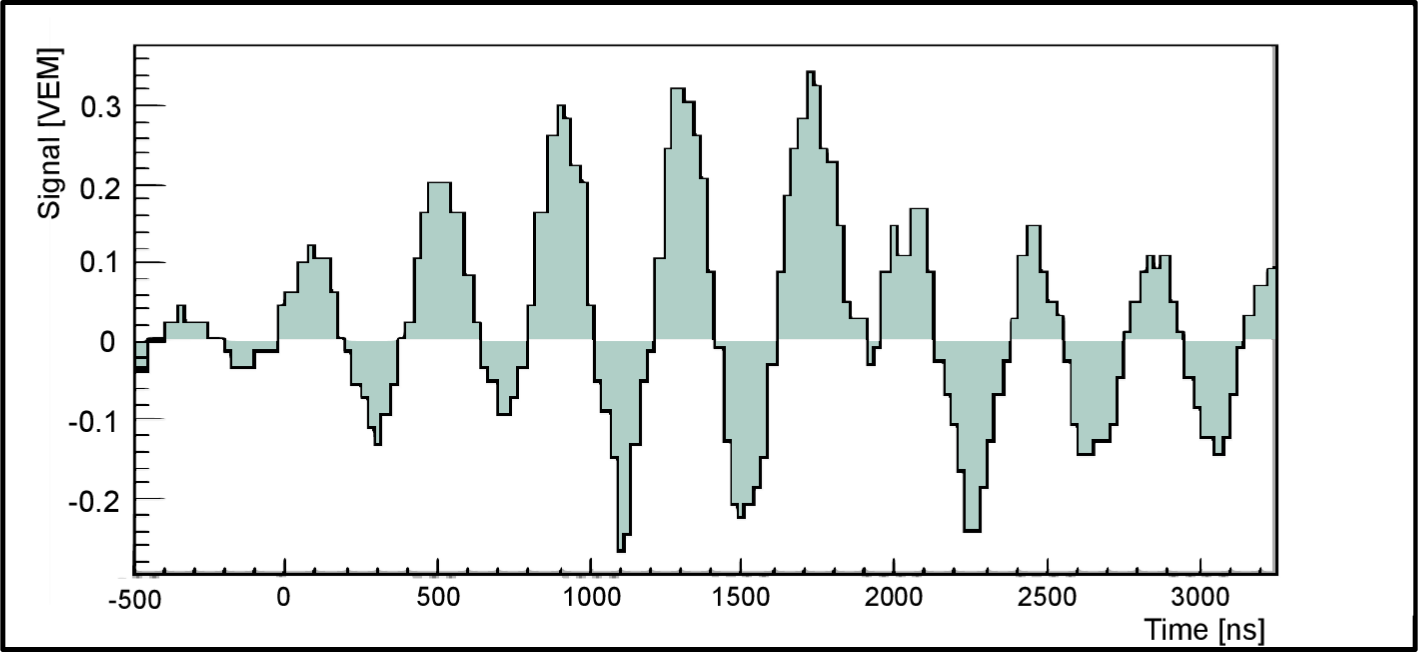
\includegraphics[height=0.35\textwidth]{fig/seleccionAuger/lighting}}
 \onslide<3>\centerline{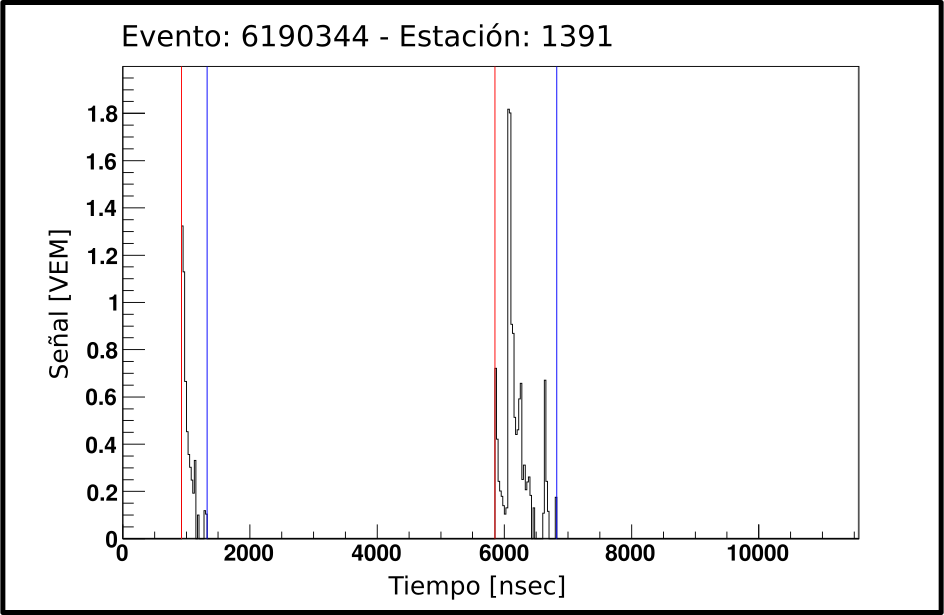
\includegraphics[height=0.35\textwidth]{fig/seleccionAuger/badStartTime}}
 \onslide<4>\centerline{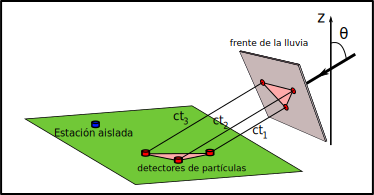
\includegraphics[height=0.35\textwidth]{fig/seleccionAuger/geome2}}
 \end{overprint}
\end{exampleblock}
\end{frame}


\begin{frame}{Selecci\'on de lluvias inclinadas}
	\begin{center}
		\begin{textblock}{6.5}(0.4,3)
% 			\begin{block}{Variables:}
			\begin{overprint}
			\onslide<1>\centerline{\pgfimage[width=1.0\textwidth]{fig/seleccionAuger/L_W_0.pdf}}
			\onslide<2->\centerline{\pgfimage[width=1.0\textwidth]{fig/seleccionAuger/L_W.pdf}}
			\end{overprint}
% 			\end{block}
		\end{textblock}
		
		\begin{textblock}{8.1}(7.4,2.5)
% 			\begin{alertblock}{}
			\begin{overprint}
			\onslide<1>\centerline{\pgfimage[height=0.65\textwidth]{fig/seleccionAuger/huellas}}
			\onslide<2->\centerline{\pgfimage[height=0.65\textwidth]{fig/seleccionAuger/sigSpeed2}}

% 			\onslide<2>
% 				\begin{tabular}{c c}
% 				Lluvia vertical & Lluvia horizontal\\
% 				$ \Delta T_{ij}\approx 0 \rightarrow V\gg c$ &$ V \approx c$\\
% 				\end{tabular}
% 				\pgfimage[width=\textwidth]{fig/seleccionAuger/sigSpeed.pdf}
			\end{overprint}
% 			\end{alertblock}
		\end{textblock}
		\begin{textblock}{15}(0.5,10.0)
			\begin{exampleblock}{}<3>
			\renewcommand{\arraystretch}{1.4}
			\scriptsize
			\centering
			\begin{tabular}{|l|c|c|c|}
			\hline
			Búsqueda & Earth-skimming (ES)           & Downward-going                        & Downward-going                       \\
					&                               & {\it high} angle (DGH)                & {\it low} angle (DGL)                \\
			\hline
						& $-$                             & $\theta_{\rm rec}>$ 75$^{\circ}$   &   $\theta_{\rm rec}\in (58.5^\circ,~76.5^{\circ})$\\
			Lluvias    & $L/W > 5$                                         & $L/W > 3$ & $-$ \\
			Inclinadas & $\langle V\rangle\in (0.29,~0.31)~{\rm m~ns^{-1}}$ & $\langle V \rangle~<~0.313~{\rm m~ns^{-1}}$ & $-$ \\
					& RMS($V$)$~<~0.08~{\rm m~ns^{-1}}$                 & RMS($V$)/$\langle V\rangle<0.08$ & $-$ \\
					& Conf 1 si $N_{ST}=3$ & & \\
			\hline
			\end{tabular}
			\end{exampleblock}
		\end{textblock}
	\end{center}
\end{frame}

\begin{frame}{Selecci\'on de lluvias j\'ovenes}
	\begin{center}\footnotesize
		\begin{textblock}{7.3}(0.4,2.)
			\begin{block}{Disparo Time over threshold (ToT)}
			
			{\footnotesize 13 bines sobre 0.2 VEM en una ventana de 3$\mu {\rm s}$}\\
			Ejemplo:
			\begin{center}
			\pgfimage[width=0.8\textwidth]{fig/seleccionAuger/traza_tot_m}
			\end{center}
			Se\~nales extendidas en el tiempo generan disparos ToT 
			\end{block}
		\end{textblock}
		
		\begin{textblock}{7.3}(8.3,2.)
			\begin{block}{Area sobre pico (AoP)}
			\begin{center}
			\pgfimage[width=0.81\textwidth]{fig/seleccionAuger/AoP_def}
			\end{center}
			Se\~nales angostas generan ${\rm AoP}\sim 1$
			\end{block}
		\end{textblock}
		
% 		\begin{textblock}{5.9}(6.4,0.6)
% 			\begin{block}{Area over peak (AoP)}
% 				\pgfimage[width=\textwidth]{fig/aopDef2.png}
% 				
% 				Narrow signals in time lead to AoP $\sim1$
% 			\end{block}
% 		\end{textblock}
		\begin{textblock}{15}(0.5,10.0)
			\begin{exampleblock}{}<2>
				\begin{center}
					{\scriptsize
					\renewcommand{\arraystretch}{1.3}
						\begin{tabular}{|c|c|c|}
						\hline
						Earth-Skimming (ES)          & Down-going High (DGH)    & Down-going Low (DGL)                       \\
						\hline\hline
						Data: 1 enero 04 - 31 mayo 10 &                                      & $\geq 75\%$ de las estaciones cerca \\
						$\geq 60\%$ de las estaciones con  &                                      & del core con ToT trigger  \\
						ToT trigger \& AoP $>$ 1.4    & Discriminante de Fisher basado             &      \&                      \\
						\cline{1-1}
						Data: 1 junio 10 - 20 junio 2013   & on AoP of {\it early} stations  & Discriminante de Fisher basado  \\
						$\langle {\rm AoP} \rangle> 1.83$  &                                 &  en el AoP de las estaciones \\
						AoP$_{\rm min}$ $>$ 1.4 if Nst=3   &                                 & tempranas cercanas al core         \\
						\hline
						\end{tabular}
					}
				\end{center}
			\end{exampleblock}
		\end{textblock}
	\end{center}
\end{frame}

\begin{frame}
 \frametitle{Selecci\'on de lluvias j\'ovenes}
 \begin{block}{Discriminante de Fisher}
 \centering
  \pgfimage[width=0.85\textwidth]{fig/seleccionAuger/ideaFisher}
 \end{block}
\end{frame}

\begin{frame}
 \frametitle{Selecci\'on de lluvias j\'ovenes}
 \framesubtitle{Ejemplo: AoP promedio (an\'alisis ES)}
	\begin{center}
	\pgfimage[width=0.9\textwidth]{fig/seleccionAuger/AoP_new_without_search_0.pdf}<1>
	\pgfimage[width=0.9\textwidth]{fig/seleccionAuger/estimaBackground.pdf}<2>
	\pgfimage[width=0.9\textwidth]{fig/seleccionAuger/AoP_new_without_search_1.pdf}<3->
	\end{center}
	
	\begin{textblock}{4.3}(7.3,8.5)
		\begin{alertblock}{}<only@3>
		\centering
	         Eficiencia de selecci\'on $\sim 90\%$	
		\end{alertblock}
	\end{textblock}
	
\end{frame}


\section[Exposicion]{C\'alculo de la exposici\'on}

\begin{frame}
 \frametitle{Estrategia de cada b\'usqueda}
 \begin{center}
  \pgfimage[width=0.9\textwidth]{./fig/estrategiaAuger/analysisSchema_4}
 \end{center}
\end{frame}

\begin{frame}
 \frametitle{C\'alculo de la exposici\'on ${\cal E}(E_\nu)$}\footnotesize
 
 \begin{exampleblock}{Definici\'on}
%  \scriptsize
 \begin{displaymath}
 N_{esp}=\int\limits_{\mathbf{E_{\nu}}}~\Phi(E_{\nu}){\cal E}(E_\nu)~dE_\nu
 \end{displaymath}
 \end{exampleblock}

 \begin{block}{Exposici\'on a neutrinos DG}
 \scriptsize
	\begin{displaymath}
	 {\cal E}_{DG}(E_\nu)\equiv\iint\limits_{\mathbf{D}~\mathbf{\Omega}}
	 {\color<2->{Red}
	 P(D|E_{\nu},\Omega)~
	 }
	 {\color<3>{Green}
	 \left[~
	 \iint\limits_{T~A}\epsilon(E_{\nu},\Omega,D,\vec{r},t)~d\vec{r}~dt
	 \right]
	 }
	 ~d\Omega~dD
	\end{displaymath}
 \end{block}
 \begin{block}{Exposici\'on a neutrinos ES}
 \scriptsize
%   \footnotesize
	\begin{displaymath}
	 {\cal E}_{ES}(E_\nu)\equiv\iiint\limits_{\mathbf{E_\tau}~\mathbf{x_d}~\mathbf{\Omega}}
	 {\color<2->{Red}
	 P({\rm x_d},E_\tau|E_{\nu},\Omega)~
	 }
	 {\color<3->{Green}
	 \left[~
	 \iint\limits_{T~A}\epsilon(E_\tau,\Omega,{\rm x_d},\vec{r},t)~d\vec{r}~dt
	 \right]
	 }
	 ~d\Omega~d{\rm x_d}~dE_\tau
	\end{displaymath}
 \end{block}
 
 \begin{block}{Interpretaci\'on}
	\begin{itemize}
	\item<2-> {\color{Red} Probabilidad de que un neutrino inicie una lluvia.}
	\item<3> {\color{Green} Probabilidad de detectar la lluvia, integrada en tiempo y \'area.}
	\end{itemize}
 \end{block}
\end{frame}
% 
\begin{frame}{T\'erminos de probabilidad}
\footnotesize
 \begin{block}{Lluvias DG}
  \centering
	\begin{itemize}
	 \item Probabilidad de que un $\nu_x$ genere una lluvia a una profundidad $D$ en la atm\'osfera:
			$$
			P(D|E_{\nu},\theta) = \frac{1}{m}~\sigma(E_{\nu})\cos\theta
			$$
	\end{itemize}
 \end{block}
 
 \begin{textblock}{3.}(1.5,9)
  \scriptsize
  \begin{alertblock}{$f(E_\tau|E_\nu,\theta)$:}
  \centering
	Obtenida mediante Monte Carlo
  \end{alertblock}
 \end{textblock}
 
 \begin{block}{Lluvias ES}
  \begin{enumerate}
   \item Probabilidad de que un $\nu_\tau$ genere un $\tau$:
	\begin{center}
		\pgfimage[width=0.45\textwidth]{./fig/exposicionAuger/pdfs_defensa}
	\end{center}
   \item Probabilidad de que el $\tau$ decaiga en en la atm\'osfera y genere una lluvia:
   \begin{displaymath}
    h(x_d,(E_\tau,\theta))=
		\exp{\left(
		-\frac{x_d}{|\cos\theta|\lambda(E_\tau)}
		\right)}
		\frac{1}{|\cos\theta|\lambda(E_\tau)}
   \end{displaymath}
  \end{enumerate}
 \end{block}
\end{frame}



\begin{frame}{Exposici\'on combinada}
	\begin{alertblock}{}
		\begin{center}
			\textbf{La muestra de datos es escrutada con los tres criterios}
		\end{center}
	\end{alertblock}
	\begin{block}{M\'etodo de combinaci\'on}
		\begin{center}
		\pgfimage[width=0.75\textwidth]{fig/exposicionAuger/sketch_combined_5}
		\end{center}
	\end{block}
\end{frame}

\begin{frame}{Exposici\'on combinada}
	\begin{block}{Resultado}
		\begin{center}
		\pgfimage[width=0.75\textwidth]{fig/exposicionAuger/exposure_combined_ageing}
		\end{center}
	\end{block}
	\begin{alertblock}{}
		\begin{center}
			\textbf{El canal ES domina por debajo de $\mathbf{10^{19}{\rm\ \mathbf{eV}}}$}
		\end{center}
	\end{alertblock}
\end{frame}
% 

\begin{frame}{Exposici\'on combinada}
\framesubtitle{Escenario $\Phi\propto E^{-2}$}
	\begin{exampleblock}{Distribuci\'on de la exposici\'on}
		\begin{center}
		\begin{tabular}{|c|c|c|c|c|}
			\hline
			\diagbox{Lluvia}{Criterio} & ES & DGH & DGL  & Total\\ \hline
			ES     &    \alert<2>{0.80}& \alert<2>{0.04} & $<0.001$ & \alert<1>{0.84} \\ \hline
			DGH    &    \alert<3>{0.03}       &    \alert<3>{0.11}       &     $<0.001$ & \alert<1>{0.14} \\ \hline
			DGL    &    $<0.001$   &    $<0.001$   &     0.02     & \alert<1>{0.02} \\
			\hline
		\end{tabular}
		\end{center}
	\end{exampleblock}
	
	\begin{block}{}
	 \begin{itemize}[<+->]
	  \item Earth Skimming domina la detecci\'on
	  \item El criterio de DGH recupera un $4\%$ de exposici\'on a eventos ES
	  \item El criterio ES recupera un $3\%$ de exposici\'on a eventos DGH
	 \end{itemize}
	\end{block}

	
\end{frame}

\begin{frame}{Errores sistem\'aticos}
	\begin{block}{Errores sistem\'aticos}
		\begin{center}
			\renewcommand{\arraystretch}{1.4}
			\scriptsize
% 			\newcolumntype{C}[1]{>{\centering\arraybackslash}p{#1}}
				\begin{tabular}{|C{0.2\textwidth}|c|c|c|c|}
% 				\begin{tabular}{|l|c|c|c|c|}
				\hline
				Fuente del  & ES        & DGH       & DGL        & Combinaci\'on         \\
				sistemático & ($90^\circ,95^\circ$) & ($75^\circ,90^\circ$) & ($65^\circ,75^\circ$) & ES / DGH / DGL   \\
		% 		\hline
		% 		& {\tiny \bf GAP 2013-100}     & \multirow{2}{*}{\tiny \bf PRD 84, 2011}    &   \multirow{2}{*}{\tiny \bf GAP2013-013} & \multirow{2}{*}{\tiny \bf 83.9\% / 13.7\% / 2.4\% }\\
		% 		& {\tiny \bf PRD 79, 2009}     &     &  &  \\
				\hline
				
				Gen. de interacción primaria    &  no apl. &   0\%, -7\%     &   +3\%, -4\%  & +0.07\%, -1.0\% \\
				
				\hline
				
				PDF en el generador             &  no apl. &   0\%, -7\%     &   +4\%, -5\%  & +0.1\%, -1.0\% \\
				
				\hline
				
				Simulador de EAS                &  no eval. &   0\%, -17\%    &   +17\%, 0\%  & +0.4\%, -2.3\% \\
				
				\hline
				
				Modelo hadrónico                & +4.7\%, -1\%      &  +5\%, -2\%     &   +0\%, -6\%  & +4.6\%, -1.3\% \\
				
				\hline
				Algoritmo de thinning           & +0.3\%, 0\%   &  +7\%,  0\%     &   +7\%,  0\%  & +1.1\%, -0.0\% \\
				\hline
				\hline
				\multirow{2}{*}{\bf $\bm{ \sigma_{\nu_\tau}\ \otimes\ \tau}$ E-loss}    & \multirow{2}{*}{\textcolor{Red}{+40\%, -33\%}}  & \multirow{2}{*}{+9\%, -9\%}  & \multirow{2}{*}{+7\%, -7\%} & \multirow{2}{*}{\bf +35\%, -29\%} \\
													&                 &                 &             & \\
				\hline
				\hline
		% 				%%%%%%%%%%%%%%%%%%%%%%%%%%%%%%%%%%%%%%%%%%%%%%%%%%%%%%%%%%%%%%%%%%%%%%%%%%%%%%%%%%%%%%%%%%%%%%%%%%
				Topography          &  +18\%, 0\%    & +24\%, 0\% & not apl.   & +18\%, 0\%  \\
				\hline
				\hline
				{\bf Total}                     &  \multicolumn{3}{c|} {}  & {\bf +39\%, -29\%}         \\
				\hline
				%%%%%%%%%%%%%%%%%%%%%%%%%%%%%%%%%%%%%%%%%%%%%%%%%%%%%%%%%%%%%%%%%%%%%%%%%%%%%%%%%%%%%%%%%%%%%%%%%%
				\end{tabular}
		\end{center}
	\end{block}
% 	\begin{exampleblock}{}
% 		\begin{center}\footnotesize
% 			La combinaci\'on se obtuvo teniendo en cuenta la contribuci\'on relativa de cada canal a la exposici\'on y correlaci\'on total.
% 		\end{center}
% 	\end{exampleblock}
\end{frame}
\section[Resultados]{B\'usqueda de candidatos y resultados}

\begin{frame}
 \frametitle{Estrategia de cada b\'usqueda}
 \begin{center}
  \pgfimage[width=0.9\textwidth]{./fig/estrategiaAuger/analysisSchema_5}
 \end{center}
\end{frame}

\begin{frame}{Unblinding DGL}
	\begin{center}
	\pgfimage[width=0.75\textwidth]{fig/resultadosAuger/DGL_Unblinding_Thesis}
	\end{center}
	\begin{block}{}
	\centering {\Large \color{red}\bf 0 candidatos}
	\end{block}
\end{frame}

\begin{frame}{Unblinding DGH}
	\begin{columns}[T]
	\column{.5\textwidth}
	\begin{tabular}{c}
	\pgfimage[width=\textwidth]{fig/resultadosAuger/DGH_Retrining_May2012_2_low_Nor_mod}\\
	\pgfimage[width=\textwidth]{fig/resultadosAuger/DGH_Retrining_May2012_2_med_Nor_mod}
	\end{tabular}

	\column{.5\textwidth}
	\pgfimage[width=\textwidth]{fig/resultadosAuger/DGH_Retrining_May2012_2_high_Nor_mod} 
	\vspace*{1cm}
	\begin{block}{}
	\centering \Large \bf \alert{0 candidatos}
	\end{block}
	\end{columns}
\end{frame}

\begin{frame}{Unblinding ES}
	\begin{center}
	\pgfimage[width=0.75\textwidth]{fig/resultadosAuger/Unblinding_ES_200613_mod}
	\end{center}
	\begin{block}{}
	\centering {\Large \color{red}\bf 0 candidatos}
	\end{block}
\end{frame}

\begin{frame}
 \frametitle{Estrategia de cada b\'usqueda}
 \begin{center}
  \pgfimage[width=0.9\textwidth]{./fig/estrategiaAuger/analysisSchema_6}
 \end{center}
\end{frame}

\begin{frame}{L\'imite al flujo de neutrinos hasta el 20 Jun 13}
	\scriptsize
		\begin{textblock}{15}(0.5,2.3)
			\begin{alertblock}{C\'alculo del l\'imite}
				\centering
				Asumiendo $\nu$ flux: $\Phi_\nu ~ = ~ k ~ E_\nu^{-2}$ $\Rightarrow$ $k_{\rm up} = \frac{N_{\rm up}}{\int_{E_{\rm min}}^{E_{\rm max}}~E_{\nu}^{-2}~{\cal E}_{\rm tot}(E_\nu)~dE_\nu}$
				\\
				M\'etodo de Conrad $\Rightarrow$ $N_{\rm up} = 2.39$
			\end{alertblock}
		\end{textblock}	
		
		\begin{textblock}{9}(0.5,5.5)
			\begin{block}{Limits}<2->
			\begin{overprint}
				\onslide<2->\centerline{\pgfimage[width=\textwidth]{fig/resultadosAuger/diff_limits_and_models_paper_combined_all_Mod}}
			\end{overprint}
			\end{block}
		\end{textblock}
		
		\begin{textblock}{5.6}(10,8)
			\begin{exampleblock}{Remarks}<3->
				\begin{itemize}
				\item Most stringent upper bound to the flux
				\item Lower than Waxman-Bachall upper bound
				\item Best sensitivity where models predict bigger fluxes
				\end{itemize}
			\end{exampleblock}
		\end{textblock}
% 		
		\begin{textblock}{5.6}(10,6)
			\begin{alertblock}{}<2->
			\centering
			\tiny
			$\bm{ k_{\rm up}=6.4 \times 10^{-9}~{\rm GeV~cm^{-2}~s^{-1}~sr^{-1}}}$
			\\ a $90\%$ C.L. $1.0\times10^{17}~{\rm eV}<E<2.5\times10^{19.5}~{\rm eV}$
			\end{alertblock}
		\end{textblock}
% % 		\begin{block}{Integrated limit}
% % 		\centering
% % 		$k_{\rm up}=6.54 \times 10^{-9}~{\rm GeV~cm^{-2}~s^{-1}~sr^{-1}}$ at $90\%$ C.L. in $10^{17}~{\rm eV}<E<10^{19.5}~{\rm eV}$
% % 		\end{block}
\end{frame}

\begin{frame}
	\frametitle{Resultados}
		\scriptsize
		\begin{block}{Rate de eventos esperado}
			\begin{center}
				\renewcommand{\arraystretch}{2.0}
				\begin{tabular}{l c c} 
	\hline
	Modelo para       &  Número esperado de eventos     & ~Probabilidad de   \\
	el flujo difuso   &  (1 enero 2004 - 20 junio 2013) & ~observar $0$   \\
	\hline
	Cosmogénico - proton, FRII \cite{Kampert_GZK}     &  $\sim$ 4.0  & $\sim 1.8\times 10^{-2}$ \\

	Cosmogénico - proton, SFR \cite{Kampert_GZK}      &  $\sim$ 0.9  & $\sim 0.4$               \\

	Cosmogénico - proton, Fermi-LAT \cite{Ahlers_GZK} &  $\sim$ 3.2  & $\sim 4\times 10^{-2}$   \\

	Cosmogénico - band \cite{Kotera_GZK}              &  $\sim$ 0.5 $-$ 1.4 & $\sim 0.6~-~0.2$ \\

	Cosmogénico - iron, FRII \cite{Kampert_GZK}       &  $\sim$ 0.3  & $\sim 0.7$ \\

	\hline

	Astrofísico $\nu$ (AGN) \cite{Becker_AGN}     &  $\sim$ 7.2  & $\sim 7\times 10^{-4}$ \\

% 	\hline
% 
% 	Exótico \cite{Sigl}                               &  $\sim$ 31.5  & $\sim 2\times 10^{-14}$ \\

	\hline
	\end{tabular}
			\end{center}
		\end{block}
		\begin{alertblock}{}
			\begin{itemize}
			 \item Optimistic proton fluxes discarted $>90\%\rm C.L.$ (\textcolor{Red}{Red numbers})
			 \item Getting close to less optimistic proton fluxes (\textcolor{Blue}{Blue numbers})
			 \item Still far from iron fluxes
			\end{itemize}
		\end{alertblock}
	\end{frame}
% 	
	\begin{frame}{Comentarios finales de la primera parte}
		\begin{center}
		\pgfimage[width=0.75\textwidth]{fig/resultadosAuger/diff_limits_and_many_models_IceCube_data_noextrap}
		\end{center}
		\begin{block}{}
		 \centering
		 \textbf{Desafio para la pr\'oxima generaci\'on de detectores de neutrinos}
		\end{block}
	\end{frame}

\part{Detecci\'on de neutrinos ultra energ\'eticos con un arreglo de antenas de radio}
\section{Introducci\'on}

\begin{frame}
\frametitle{Introducci\'on}
 \footnotesize
 \begin{exampleblock}{Principio de detecci\'on}
  \centering
  \textbf{La componente electromagn\'etica de lluvias emiten se\~nales de radio\\ \alert{$\bm\Rightarrow$ Se pueden medir con un arreglo de antenas}}
 \end{exampleblock}
 
 \begin{alertblock}{Esta parte de la tesis:}<+->
  Estimar el desempe\~no de un arreglo de 90000 antenas de radio al detectar $\nu$ ES.
 \end{alertblock}
 
 \begin{block}{Resumen:}<+->
  \begin{itemize}[<alert@+>]\setlength\itemsep{2mm}
   \item Emisi\'on de ondas de radio por lluvias atmosf\'ericas.
   \item Simulaci\'on de lluvias hadr\'onicas y de neutrinos ES.
   \item C\'alculo de la eficiencia y la exposici\'on.
   \item L\'imite esperado y comparaci\'on con Auger y otros experimentos.
  \end{itemize}
 \end{block}
% 
\end{frame}

% Hay otro mecanismo para detectar lluvias atmosfericas (hadronicas o de neutrinos)
% La componente electromagnetica de las lluvias emite ondas de radio
% => se pueden medir con un arreglo de antenas
% En esta parte estudio la factibilidad de buscar neutrinos ES por este metodo 
% Resumen:
% 1. emision de ondas de radio por lluvias atmosfericas 
% 2. simulacion para lluvias hadronicas y para neutrinos ES
% 3. calculo de la eficiencia y la exposicion
% 4. limite esperado y comparacion con Auger y otros experimentos

\begin{frame}
 \frametitle{Motivaci\'on}
 \footnotesize

 
 \begin{block}{?`Por qu\'e un arreglo de antenas de radio?}<+->
  \begin{itemize}\setlength\itemsep{3mm}
   \item La amplitud del pulso posee informaci\'on sobre  $N_{max}\propto E_{prim}$
   \item La estructura temporal guarda informaci\'on sobre la distribuci\'on longitudinal de la lluvia $\rightarrow\ X_{max}$
   \item Casi $100\%$ de tiempo de operaci\'on.
   \item Bajo costo relativo.
  \end{itemize}
 \end{block}
 
 \begin{exampleblock}{GRAND}<+->
  Propone desplegar 90000 antenas en Tianshian, China para desarrollar b\'usquedas de neutrinos c\'osmicos ultra energ\'eticos.
 \end{exampleblock}
 
\end{frame}

\section[Emisi\'on]{Emisi\'on de radio en EAS}

\begin{frame}{Emisi\'on de radio en lluvias atmosf\'ericas}
\framesubtitle{Mecanismos de emisi\'on - Polarizaci\'on}
\footnotesize
	
	\begin{alertblock}{}
	\centering
	\textbf{?`c\'omo emiten? }$\rightarrow$ Superposici\'on de se\~nales
	\end{alertblock}
	
	\begin{exampleblock}{Dos mecanismos efectivos}<+->
		\begin{itemize}[<alert@+|+->]
		 \item Efecto geomagn\'etico
		 \item Efecto Askaryan
		\end{itemize}
	\end{exampleblock}
	\vfill
	\begin{overprint}
	\onslide<2>
		\centerline{\pgfimage[width=0.8\textwidth]{fig/EASRadio/geom_sketch}}
	\onslide<3>
		\centerline{\pgfimage[width=0.8\textwidth]{fig/EASRadio/ask_sketch}}
	\end{overprint}
\end{frame}

% \begin{frame}{Emisi\'on de radio en lluvias atmosf\'ericas}
% \footnotesize
% 	\begin{block}{}
% 		\begin{center}
% 		
% 		\end{center}
% 	\end{block}
% \end{frame}

\begin{frame}{Emisi\'on de radio en lluvias atmosf\'ericas}
\framesubtitle{Huella y estructura temporal}
\footnotesize
	\begin{block}{\'Angulo Cherenkov}
		\begin{overprint}
		\onslide<1>\centerline{\pgfimage[width=0.9\textwidth]{fig/EASRadio/aminCher/cono_1}}
		\onslide<2>\centerline{\pgfimage[width=0.9\textwidth]{fig/EASRadio/aminCher/cono_2}}
		\onslide<3>\centerline{\pgfimage[width=0.9\textwidth]{fig/EASRadio/aminCher/cono_3}}
		\onslide<4>\centerline{\pgfimage[width=0.9\textwidth]{fig/EASRadio/aminCher/cono_4}}
		\onslide<5>\centerline{\pgfimage[width=0.9\textwidth]{fig/EASRadio/aminCher/cono_5}}
		\onslide<6>\centerline{\pgfimage[width=0.9\textwidth]{fig/EASRadio/aminCher/cono_6}}
		\onslide<7>\centerline{\pgfimage[width=0.9\textwidth]{fig/EASRadio/chConeSch}}
		\end{overprint}
	\end{block}
	\begin{alertblock}{}
		\begin{overprint}
		\onslide<1-6>
			\centerline{\textbf{$n\sim1.000325$ $\rightarrow$ $\theta_{cher}\sim1.4^\circ$}}
		\onslide<7>
			\centerline{\alert<7>{\textbf{Anillo Cherenkov}}}
		\end{overprint}
	\end{alertblock}
\end{frame}

\begin{frame}{Geometr\'ia del cono Cherenkov}
\framesubtitle{Eventos ES}
\footnotesize
	\begin{block}{Esquema}
		\begin{center}
		\pgfimage[width=0.9\textwidth]{fig/modeloRadio/coneProy}
		\end{center}
	\end{block}
	\begin{alertblock}{Intersecci\'on del cono Cherenkov sobre el suelo: hip\'erbola}
		\begin{center}
		 \begin{displaymath}
			w^2(d)=
			(\tan^2 \theta_{cher}-\tan^2 (\theta-\frac{\pi}{2}))
			(\frac{d}{\sin \theta}-l_{max})^2
			- \tan (\theta-\frac{\pi}{2}) \frac{h_{max}}{\sin \theta} (\frac{d}{\sin \theta}-l_{max})
			- \frac{h_{max}^2}{\sin^2 \theta}
		 \end{displaymath}
		\end{center}
	\end{alertblock}
\end{frame}
% \section[Modelado]{Modelado Radio}

\begin{frame}{Modelo de juguete}
\footnotesize
	\begin{exampleblock}{Esquema}
		\begin{center}
		\pgfimage[width=0.85\textwidth]{fig/modeloRadio/timeDelaySchema}
		\end{center}
	\end{exampleblock}
	\begin{block}{Resultado}<2>
		\begin{center}
		\visible<2>{
		\pgfimage[height=0.25\textwidth]{fig/modeloRadio/timeDelay_pd} \hspace*{0mm}
		\pgfimage[height=0.25\textwidth]{fig/modeloRadio/legend.pdf} \hspace*{0mm}
		\pgfimage[height=0.25\textwidth]{fig/modeloRadio/timeDelay_spa} \hspace*{0mm}
		}
		\end{center}
	\end{block}
\end{frame}

\section[Simulaci\'on]{Simulaci\'on Radio}



\begin{frame}{Cadena de simulaci\'on}
\footnotesize
	\begin{block}{Etapas}
		\begin{center}
		\pgfimage[width=0.9\textwidth]{fig/simulacionRadio/sim_cartoon_upgoing}
		\end{center}
	\end{block}
% 	\begin{alertblock}{Caracter\'isticas deseables}
% 	\end{alertblock}
\end{frame}



\begin{frame}{Representaci\'on del detector}
\footnotesize
	\begin{block}{Esquema del detector}
		\begin{center}
		\pgfimage[width=0.6\textwidth]{fig/simulacionRadio/antennaSch.pdf}
		\end{center}
	\end{block}
	\begin{alertblock}{Antena sobre el cono Cherenkov}
	\begin{center}
		\pgfimage[width=0.48\textwidth]{fig/simulacionRadio/antennaSignal}\hspace*{2mm}
		\pgfimage[width=0.48\textwidth]{fig/simulacionRadio/antennaFilt}
	\end{center}
	\end{alertblock}
\end{frame}

\begin{frame}{Disparo local}
\footnotesize
	\begin{exampleblock}{Fuentes}
	\begin{itemize}
	 \item Ionosf\'erico
	 \item Proveniente de la ciudad
	 \item Gal\'actico
	 \item Intr\'inseco
	\end{itemize}
	\end{exampleblock}
	\begin{block}{Intensidad}
		\begin{center}
		\pgfimage[width=0.5\textwidth]{fig/simulacionRadio/allanNoise.pdf}
		\end{center}
	\end{block}
	\vspace*{-1cm}
	\begin{alertblock}{}
		\begin{center}
		\textbf{Nivel de disparo local entre \cant{\bm{40}}{\bm{\mu V/m}} y \cant{\bm{25}}{\bm{\mu V/m}}}
		\end{center}
	\end{alertblock}
\end{frame}

\section[Caracter\'isticas]{Caracterizaci\'on}

\begin{frame}{Caracter\'isticas de la huella}
\footnotesize
	\begin{block}{Huella del m\'aximo de campo el\'ectrico - $\theta=90.5^\circ$\cant{}{x_d=25m} \cant{E_v=10^{18}}{eV} $\phi=90^\circ$}
		\begin{center}
		\pgfimage[width=0.85\textwidth]{fig/caracterizacionRadio/foorPrint_Cone_ZWv1.22_ntuples_v1.21_ChTest_phi_90_18_89.5_90_25_1238_E0.png}
		\end{center}
	\end{block}
	\begin{alertblock}{}
	 \begin{itemize}
	  \item Huella descripta por la ecuaci\'on de la hip\'erbola
	  \item Se\~nales largas y angostas
	 \end{itemize}
	\end{alertblock}
\end{frame}

\begin{frame}{Caracter\'isticas de la huella}
\footnotesize
% 	\begin{block}{Distribuci\'on de part\'iculas}
	\begin{center}
	\pgfimage[width=0.85\textwidth]{fig/caracterizacionRadio/foorPrint_Test_18_89-5_90_25_1238_E_particles_2}
	\end{center}
	\begin{alertblock}{}
	 \begin{itemize}
	  \item La huella de radio es mucho m\'as extensa que la distribuci\'on de part\'iculas.
	  \item Permite espaciar las estaciones
	 \end{itemize}
	\end{alertblock}
\end{frame}



% \begin{frame}{Caracterizaci\'on}
% \footnotesize
% 	\begin{block}{Capacidad de disparo}
% 		\begin{center}
% 		Mostrar cortes en distintas variables
% % 		\pgfimage[width=0.85\textwidth]{fig/caracterizacionRadio/phiDist_Test_18_89.5_90_25_1238}
% 		\end{center}
% 	\end{block}
% \end{frame}

% \begin{frame}{Espacio de par\'ametros simulado}
% \footnotesize
% 	\begin{block}{Capacidad de disparo}
% 		\begin{center}
% 		\pgfimage[width=0.85\textwidth]{fig/caracterizacionRadio/binesRadio_3}
% 		\end{center}
% 	\end{block}
% \end{frame}
\section[Exposicion]{C\'alculo de la exposici\'on}

\begin{frame}{C\'alculo de exposici\'on}
\footnotesize
		\begin{block}{F\'ormula}
			\begin{center}
			\begin{displaymath}
			\begin{aligned}
				{\cal E} (E_\nu) = 2 \pi 
				\textcolor{Red}{T A}
				\int_{0}^{\infty} 
				\int_{\theta^{cut}}^{\theta^{max}} 
				\int_{0}^{E_\nu} 
				\int_{0}^{E_\tau} 
				\textcolor<2->{Blue}{\epsilon (x_d,\theta,E_{sh})}
				\textcolor<3->{DarkOrange}{
				\frac{e^{-\frac{l(x_d)}{\lambda(E_\tau)}}}{\lambda(E_\tau)}\frac{dl(x_d)}{dx_d}
				}
				\textcolor<4->{DarkViolet}{P(E_{sh}|E_\tau)}\\
				\textcolor<5->{Green}{P(E_\tau|E_\nu,\theta)}
				\textcolor<6->{Magenta}{\sin \theta \cos \theta}
				dE_{sh} dE_\tau  d\theta dx_d
			\end{aligned}
		\end{displaymath}
			\end{center}
		\end{block}
		\begin{exampleblock}{Ingredientes}
			\begin{itemize}[<+->]
			 \item \textcolor{Red}{Tiempo de medici\'on y \'area del detector.}
			 \item \textcolor{Blue}{Eficiencia de detecci\'on.}
			 \item \textcolor{DarkOrange}{Probabilidad de decaimiento de un $\tau$ a altura ${\rm x_d}$.}
			 \item \textcolor{DarkViolet}{Probabilidad que un $\tau$ de energ\'ia $E_\tau$ produzca una lluvia de energ\'ia $E_{sh}$.}
			 \item \textcolor{Green}{Interacci\'on en la tierra.}
			 \item \textcolor{Magenta}{\'Angulo s\'olido.}
			\end{itemize}
		\end{exampleblock}
\end{frame}

\begin{frame}{Topograf\'ia del detector}
\footnotesize
	\begin{block}{Descripci\'on}
		\begin{center}
		\pgfimage[width=0.85\textwidth]{fig/resultadosRadio/topografia}
		\end{center}
	\end{block}
% 	\begin{block}{}
% 		\begin{center}
% 		
% 		\end{center}
% 	\end{block}
\end{frame}

\begin{frame}{C\'alculo de la eficiencia}
\footnotesize
	\begin{block}{Se lanz\'o cada lluvia 1000 veces sobre la celda primitiva}
	\centering
		\pgfimage[width=0.48\textwidth]{fig/resultadosRadio/17.00_89.90_00.00_00025_01238_1000_1000_90_re}\hspace*{2mm}
		\pgfimage[width=0.48\textwidth]{fig/resultadosRadio/17.00_89.90_00.00_00025_01238_1500_1500_60_re} \\ \vspace*{2mm}
		\pgfimage[width=0.48\textwidth]{fig/resultadosRadio/17.00_89.90_00.00_00025_01238_500_4000_90_de}\hspace*{2mm}
		\pgfimage[width=0.48\textwidth]{fig/resultadosRadio/17.00_89.90_00.00_00025_01238_750_750_60_hc}
	\end{block}
% 	\begin{block}{}
% 		\begin{center}
% 		
% 		\end{center}
% 	\end{block}
\end{frame}

\begin{frame}{C\'alculo de la eficiencia}
\footnotesize
	\begin{block}{Se lanz\'o cada lluvia 1000 veces sobre la celda primitiva}
	\centering
		\pgfimage[width=0.85\textwidth]{fig/resultadosRadio/trigger}
	\end{block}
% 	\begin{block}{}
% 		\begin{center}
% 		
% 		\end{center}
% 	\end{block}
\end{frame}


\begin{frame}{C\'alculo de la eficiencia}
\footnotesize
	\begin{block}{Curvas de eficiencia}
	\centering
		\pgfimage[width=0.85\textwidth]{fig/resultadosRadio/eff50.0_5.0_1000.0_1000.0_60.0_1.0_17.75_m2}
	\end{block}
% 	\begin{block}{}
% 		\begin{center}
% 		
% 		\end{center}
% 	\end{block}
\end{frame}

\begin{frame}{Eficiencias de identificaci\'on}
\footnotesize
	\begin{block}{Eventos DG dejan huellas m\'as anchas que los ES}
	\centering
		\pgfimage[width=0.48\textwidth]{fig/resultadosRadio/foorPrint_ZWv1.34_ntuples_v1.22_Downgoing_phi_90_18.5_89_90_100_5_E}\hspace*{2mm}
		\pgfimage[width=0.48\textwidth]{fig/resultadosRadio/foorPrint_Cone_ZWv1.22_ntuples_v1.21_ChTest_phi_90_18_89.5_90_25_1238_E0_u}
	\end{block}
	
	\begin{block}{Pueden ser discriminados}
	\centering
		\pgfimage[width=0.48\textwidth]{fig/resultadosRadio/idRadio}\hspace*{2mm}
		\pgfimage[width=0.48\textwidth]{fig/resultadosRadio/showerWidth_Comp_DG_ES_Wt}
	\end{block}
	
% 	\begin{block}{}
% 		\begin{center}
% 		
% 		\end{center}
% 	\end{block}
\end{frame}


\section[Resultados]{Resultado final}

\begin{frame}{Comparaci\'on con Auger}
\footnotesize
	\begin{block}{Cociente de cantidad de eventos esperados como funci\'on del threshold local}
	\centering
		\pgfimage[width=0.85\textwidth]{fig/resultadosRadio/CompRadioAuger_1000.0_5.0_1.0_de_modo3}
	\end{block}
	
% 	\begin{block}{}
% 		\begin{center}
% 		
% 		\end{center}
% 	\end{block}
\end{frame}

\begin{frame}{Comparaci\'on con Auger}
\footnotesize
	\begin{block}{Cociente de cantidad de eventos esperados}
	\centering
		\pgfimage[width=0.85\textwidth]{fig/resultadosRadio/CompRadioAuger_50.0_5.0_1.0_de_modo2}
	\end{block}
	
% 	\begin{block}{}
% 		\begin{center}
% 		
% 		\end{center}
% 	\end{block}
\end{frame}

\begin{frame}{Comparaci\'on con Auger}
\footnotesize
	\begin{block}{Tama\~no dle detector}
	\centering
		\pgfimage[width=0.85\textwidth]{fig/resultadosRadio/area/Area_de}
	\end{block}
	
% 	\begin{block}{}
% 		\begin{center}
% 		
% 		\end{center}
% 	\end{block}
\end{frame}

\begin{frame}{Comparaci\'on con Auger}
\footnotesize
	\begin{block}{Tama\~no dle detector}
	\centering
		\pgfimage[width=0.85\textwidth]{fig/resultadosRadio/area/CompRadioAuger_50.0_5.0_1.0_de_modo2}
	\end{block}
	
% 	\begin{block}{}
% 		\begin{center}
% 		
% 		\end{center}
% 	\end{block}
\end{frame}

\begin{frame}{L\'imite diferencial en 3 a\~nos de exposici\'on}

				\begin{alertblock}{\scriptsize C\'alculo del l\'imite}
				\centering
				\scriptsize
				Se asume un flujo: $\Phi_\nu ~ = ~ k ~ E_\nu^{-2}$ $\Rightarrow$ ${\text k (E_\nu)} = \frac{2.4}{\int\limits_{E_\nu-\Delta}^{E_\nu+\Delta} \tilde{E}_{\nu}^{-2}~{\cal E}(\tilde{E}_\nu) d\tilde{E}_\nu}$
			\end{alertblock}
		
		
		\begin{block}{\scriptsize L\'imite diferencial: 90000 antennas - Trigger local 50${\rm \mu Vm}$ - L = 250 ${\rm km}$ - 500${\rm km}$}
			\begin{center}
			\pgfimage[height=0.45\textwidth]{fig/resultadosRadio/limits_future_v1_2_2.pdf}
			\end{center}
		\end{block}
\end{frame}

\begin{frame}{Desempe\~no - L = 250 ${\rm km}$}
	\begin{block}{Rate de eventos}
		\begin{center}
		\renewcommand{\arraystretch}{1.3}
		\footnotesize
		\begin{tabular}{lccc}
			\hline
			\multirow{2}{*}{Modelo} & \multicolumn{3}{c}{Topograf\'ia - \cant{L=250}{km}} \\
			&   Regular &   Panal de abeja &   Bordes densos \\
			\hline
			Cosmogénico - proton, FRII &    45.3 &             52.2 &            52.5 \\
			Cosmogénico - proton, Fermi-LAT &     34.1 &             39.4 &            39.5 \\
			Cosmogénico - proton, SFR &     10.3 &             11.8 &            11.9 \\
			Cosmogénico - H\'ibrido &      5.8 - 14.9 &      6.7 - 17.2 &       6.7 - 17.3 \\
			Cosmogénico - iron, FRII &     3.2 &              3.6 &             3.7 \\
			IceCube extrapolado $E^{-2}$ &      13.1 &             15.1 &            15.2 \\
			IceCube extrapolado \emph{Best fit}  &      12.9 &             14.9 &            15   \\
			\hline
		\end{tabular}
		\end{center}
	\end{block}
\end{frame}

\begin{frame}{Desempe\~no - L = 500 ${\rm km}$}
	\begin{block}{Rate de eventos}
		\begin{center}
		\renewcommand{\arraystretch}{1.3}
		\footnotesize
		\begin{tabular}{lccc}
			\hline
			\multirow{2}{*}{Modelo} & \multicolumn{3}{c}{Topograf\'ia - \cant{L=500}{km}} \\
			&   Regular &   Panal de abeja &   Bordes densos \\
			\hline
			Cosmogénico - proton, FRII &    185.8 &            193   &           191.3 \\
			Cosmogénico - proton, Fermi-LAT &     140.3 &             146.0 &           144.8 \\
			Cosmogénico - proton, SFR &     42.1 &             43.8   &            43.4 \\
			Cosmogénico - H\'ibrido &  23.9 - 61.3 &   24.8 - 63.7 &  24.6 - 63.2 \\
			Cosmogénico - iron, FRII &     13.0   &        13.4 &            13.3 \\
			IceCube extrapolado $E^{-2}$ &      53.6 &         55.5   &            55   \\
			IceCube extrapolado \emph{Best fit} &    52.4 &  53.8  &   53.3 \\
			\hline
		\end{tabular}
		\end{center}
	\end{block}
\end{frame}


\section[Conclusiones]{Conclusiones}

\begin{frame}{Comentarios finales}
\scriptsize
	\begin{block}{}
	\centering
	\textbf{Se estudi\'o la medici\'on de neutrinos c\'osmicos ultra energ\'eticos con detectores de superficie.}
	\end{block}
	
	\begin{exampleblock}{\centering B\'usqueda de neutrinos con el observatorio Pierre Auger}
	\begin{itemize}[<alert@+|+->]
	 \item Se presentaron los procedimientos de identificaci\'on de lluvias inclinadas y j\'ovenes, y el c\'alculo de la exposici\'on asociada a las tres b\'usquedas realizadas por Auger.
	 \item Se integraron los canales de b\'usqueda en un an\'alisis combinado, teniendo en cuenta la correlaci\'on entre sistem\'aticos y las posibilidades de detecci\'on cruzada.
	 \item Se obtuvo el l\'imite integrado m\'as estricto al flujo difuso en el rango \cant{1\text{-}80}{EeV}, \cant{k<6.4\times 10^{-9}}{Gev\ cm^{-2}\ s^{-1}\ sr^{-1}} (90$\%$ C.L.) con $\Phi=k\ E^{-2}$
	 \item Se rechazaron los modelos de flujos que suponen protones como primario y una evoluci\'on optimista para las fuentes.
	\end{itemize}
	\end{exampleblock}
	
	\begin{alertblock}{\centering B\'usqueda de neutrinos con un arreglo de antenas de radio}
	\begin{itemize}[<alert@+|+->]
	 \item Se describi\'o la emisi\'on de ondas de radio por lluvias atmosf\'ericas y se realiz\'o una caracterizaci\'on de la huella dejada en la superficie por neutrinos rasantes.
	 \item Se determin\'o la eficiencia y la exposici\'on para distintas configuraciones de antenas.
	 \item Se encontr\'o que para un detector del tama\~no de GRAND es factible alcanzar una exposici\'on por unidad de tiempo un orden de magnitud mayor que la de Auger.
	 \item Esto permitir\'ia estudiar la mayor\'ia de los modelos que utilizan protones como primario e incluso alcanzar los generados por hierro.
	\end{itemize}
	\end{alertblock}

\end{frame}

\begin{frame}{}
 \begin{alertblock}{}
  \centering
  \huge{
  Muchas gracias!
  }
 \end{alertblock}
\end{frame}

\begin{frame}{Agradecimientos}
 \begin{alertblock}{}
  \begin{itemize}
   \item Fernanda
   \item Ricardo y Jaime
   \item Yann y Javier
   \item Mi familia
   \item Mis amigos
   \item Compa\~neros de trabajo
   \item La UBA
  \end{itemize}

 \end{alertblock}
\end{frame}
\section{Backup Slides}

\frame{\sectionpage}

	
\begin{frame}
\frametitle{Observatorio Pierre Auger (PAO)}
\framesubtitle{Descripci\'on}
	\begin{block}{Detector - Tama\~no}
		\begin{center}
			\pgfimage[width=0.7\textwidth]{./fig/detectorAuger/augercapfed}
		\end{center}
	\end{block}
\end{frame}

\begin{frame}{Identificaci\'on de neutrinos con el SD de Auger}
	\begin{alertblock}{}\centering
	Con el SD es posible distinguir frentes mu\'onicos de frentes electromagn\'eticos.
% 			With the SD, we can distinguish muonic from electromagnetic shower fronts (using the time structure of the signals in the water Cherenkov stations).
	\end{alertblock}
	
	\begin{block}{Traza Cherenkov medida con una resoluci\'on de 25ns}
	\centering
	\pgfimage[width=0.8\textwidth]{fig/detectorAuger/tanque_muon.pdf}
	\end{block}
	
\end{frame}

\begin{frame}
 \frametitle{Divisi\'on de las muestras para DG}
	\begin{block}{DGL}
		\begin{center}
		\pgfimage[width=0.9\textwidth]{./fig/simulacionAuger/periodosDGL}
		\end{center}
	\end{block}
	\begin{block}{DGH}
		\begin{center}
		\pgfimage[width=0.9\textwidth]{./fig/simulacionAuger/periodosDGH}
		\end{center}
	\end{block}
\end{frame}

\begin{frame}
 \frametitle{Divisi\'on de las muestras para ES}
	\begin{block}{ES}
		\begin{center}	 
		\pgfimage[width=0.9\textwidth]{./fig/simulacionAuger/periodosES}
		\end{center}
	\end{block}
\end{frame}


\begin{frame}
 \frametitle{Estrategia de cada b\'usqueda}
 \begin{center}
  \pgfimage[width=0.9\textwidth]{./fig/estrategiaAuger/analysisSchema_1}
 \end{center}
\end{frame}


\begin{frame}
 \frametitle{Selecci\'on de lluvias j\'ovenes}
 \begin{block}{Discriminante de Fisher}
 \centering
  \pgfimage[width=0.85\textwidth]{fig/seleccionAuger/ideaFisher}
 \end{block}
\end{frame}

\begin{frame}{Eficiencias DG}
	\begin{block}{Disparo com funci\'on de la prifundidad}
		\begin{center}
		\pgfimage[width=0.75\textwidth]{fig/exposicionAuger/eff_10EeV_85}
		\end{center}
	\end{block}
\end{frame}

\begin{frame}{Eficiencias DG}
	\begin{block}{Disparo com funci\'on de la energ\'ia}
		\begin{center}
		\pgfimage[width=0.75\textwidth]{fig/exposicionAuger/eff_varios_85}
		\end{center}
	\end{block}
\end{frame}

\begin{frame}{Eficiencias DG}
\footnotesize
	\begin{block}{Disparo com funci\'on del \'angulo cenital}
		\begin{center}
		\pgfimage[width=0.4\textwidth]{fig/exposicionAuger/eff_1EeV_80}\hspace{3mm}
		\pgfimage[width=0.4\textwidth]{fig/exposicionAuger/eff_1EeV_85}
		\end{center}
	\end{block}
% \end{frame}
% 
% \begin{frame}{Eficiencias DG}
	\begin{block}{Disparo com funci\'on del canal de interaccion}
		\begin{center}
		\pgfimage[width=0.4\textwidth]{fig/exposicionAuger/eff_CCvsNC_85}\hspace{3mm}
		\pgfimage[width=0.4\textwidth]{fig/exposicionAuger/eff_tau_1EeV_85}
		\end{center}
	\end{block}
\end{frame}

\begin{frame}{Eficiencias ES}
	\begin{block}{Disparo com funci\'on de la altura de decaimiento}
		\begin{center}
		\pgfimage[width=0.75\textwidth]{fig/exposicionAuger/eff_18_8931_forThesis}
		\end{center}
	\end{block}
\end{frame}

\begin{frame}{Eficiencias ES}
	\begin{block}{Disparo com funci\'on de la energ\'ia}
		\begin{center}
		\pgfimage[width=0.75\textwidth]{fig/exposicionAuger/eff_multEnergy_forThesis}
		\end{center}
	\end{block}
\end{frame}

\begin{frame}{Eficiencias ES}
\footnotesize
	\begin{block}{Disparo com funci\'on del \'angulo cenital}
		\begin{center}
		\pgfimage[width=0.48\textwidth]{fig/exposicionAuger/eff_multiTheta_forThesis}
		\hspace{1mm}
		\pgfimage[width=0.48\textwidth]{fig/exposicionAuger/eff_multTheta_h10_forThesis}
		\end{center}
	\end{block}
	\begin{block}{Definicion de la variable $h_{10}$}
		\begin{center}
		\pgfimage[width=0.45\textwidth]{fig/exposicionAuger/hc_def.pdf}
		\end{center}
	\end{block}
\end{frame}

\begin{frame}{Integraci\'on temporal y en superficie}
	\begin{block}{M\'etodo de calculo}
		\begin{center}
		\pgfimage[width=0.6\textwidth]{fig/exposicionAuger/aperturaReal}
		\end{center}
	\end{block}
\end{frame}

\begin{frame}{Integraci\'on temporal y en superficie}
	\begin{block}{Selecci\'on de la configuraci\'on del detector}
		\begin{center}
		\pgfimage[width=0.75\textwidth]{fig/exposicionAuger/t2FilePlot}
		\end{center}
	\end{block}
\end{frame}


\begin{frame}{Integraci\'on temporal y en superficie}
	\begin{block}{Envejecimiento de detector}
		\begin{center}
		\pgfimage[width=0.9\textwidth]{fig/exposicionAuger/timeEvolution_1}<1>
		\pgfimage[width=0.9\textwidth]{fig/exposicionAuger/timeEvolution_2}<2>
		\pgfimage[width=0.9\textwidth]{fig/exposicionAuger/timeEvolution_3}<3>
		\pgfimage[width=0.9\textwidth]{fig/exposicionAuger/fractionEvolution}<4>
		\end{center}
	\end{block}
\end{frame}


\begin{frame}{Integraci\'on temporal y en superficie}
	\begin{block}{Envejecimiento de detector}
		\begin{center}
		\pgfimage[width=0.55\textwidth]{fig/exposicionAuger/timedecay_vs_reflect_absorp_2}
		\end{center}
	\end{block}
	\begin{block}{Envejecimiento de detector}<2>
		\begin{center}
		\renewcommand{\arraystretch}{1.4}
		\footnotesize
		\begin{tabular}{|l|ccc|c|}
					\hline
					Período       & tyRef & wAbs & LDT        &    Pérdida de exposición \\
					\hline
					$2004 - 2008$ & 0.94  & 100  & $\sim63$ns &    $--$ \\
					$2009 - 2010$ & 0.94  & 80   & $\sim60$ns &    $-15.2\%$\\
					$2011 - 2013$ & 0.93  & 100  & $\sim57$ns &    $-17.5\%$\\
					\hline
		\end{tabular}
		\end{center}
	\end{block}
\end{frame}

\begin{frame}{Exposici\'on combinada}
	\begin{block}{Obtenci\'on de la exposicion total}
		\begin{center}
			\begin{displaymath}\renewcommand{\arraystretch}{2}
			\begin{array}{rcl}
			N_{esp}& =& N_{esp}^{DGL}+N_{esp}^{DGH}+N_{esp}^{ES} \\ 
			& = & \int\limits_{E_\nu}\Phi(E_\nu)~({\cal E}^{DGL}+{\cal E}^{DGH}+{\cal E}^{ES})(E_\nu)~dE_\nu\\
			& \equiv & \int\limits_{E_\nu}\Phi(E_\nu)~{\cal E}(E_\nu)~dE_\nu
			\end{array}
			\end{displaymath}
		\end{center}
	\end{block}
	
	\begin{alertblock}{}
	\centering
% 		\begin{center}
			\begin{displaymath}
			{\cal E}(E_\nu) = {\cal E}^{DGL}+{\cal E}^{DGH}+{\cal E}^{ES}
			\end{displaymath}
% 		\end{center}
	\end{alertblock}
	
	\begin{exampleblock}{}
		\begin{center}
			\textbf{La exposici\'on combinada es la suma de las individuales}
		\end{center}
	\end{exampleblock}
\end{frame}

\begin{frame}{Errores sistem\'aticos}
	\begin{alertblock}{Bines representativos en ES}
		\begin{center}
			\pgfimage[width=0.75\textwidth]{fig/exposicionAuger/importantBins_oldWeights}
		\end{center}
	\end{alertblock}
	\begin{block}{Resultado}
		\begin{center}
			Se recalculo la exposici\'on sobre los bines que m\'as contribuyen a la exposici\'on.
		\end{center}
	\end{block}
\end{frame}

\begin{frame}{Errores sistem\'aticos}
	\begin{block}{}
		\begin{center}
			\pgfimage[width=0.45\textwidth]{fig/exposicionAuger/nu_xsection_models}\hspace{2mm}
			\pgfimage[width=0.45\textwidth]{fig/exposicionAuger/tau_E_loss_models}
		\end{center}
	\end{block}
	\begin{exampleblock}{}
		\begin{center}
			\begin{tabular}{|l|l|l|}
			\hline
			\textbf{Modelo}      & Secci\'on eficaz& P\'erdida de energ\'ia del $\tau$ \\ 
			\hline
			Referencia &    Sarkar     & ALLM\\ 
			%
			Pesimista &  ASW &     BB\\ 
			%
			Optimista &   Armesto Sat. $\lambda=0.4$&  ASW\\
			\hline 
			\end{tabular}  
		\end{center}
	\end{exampleblock}
\end{frame}

\begin{frame}{Errores sistem\'aticos}
	\begin{block}{Cambio en las probabilidades}
		\begin{center}
			\pgfimage[width=0.75\textwidth]{fig/exposicionAuger/pdfSyst}
		\end{center}
	\end{block}
	\begin{exampleblock}{Resultado}
		\begin{center}
			Cambian la probabilidad de emerger y el espectro de energ\'ia.
		\end{center}
	\end{exampleblock}
\end{frame}


\begin{frame}{Emisi\'on de radio en lluvias atmosf\'ericas}
\framesubtitle{Origen}
\footnotesize
	
	\begin{block}{Part\'icula que se desplaza en l\'inea recta a velocidad constante}
		\begin{center}
		\pgfimage[width=0.5\textwidth]{fig/EASRadio/trackSch}
		\end{center}
	\end{block}
	
	\begin{block}{Aproximaci\'on ZHS}
		\begin{center}
		\pgfimage[width=0.5\textwidth]{fig/EASRadio/zhs_pulse}
		\end{center}
	\end{block}
\end{frame}

\begin{frame}{Ubicaci\'on del detector}
\footnotesize
	\begin{block}{Posibles ubicaciones}
		\begin{center}\scriptsize
		\begin{tabular}{LLLL}
		\toprule
		Experimento (Sitio) & Declinaci\'on (+E,-W) & Inclinaci\'on (+D,-U)& Intensidad [Gauss] \\
		\midrule
		Auger AERA (Malarg\"ue Argentina) 
% 		& $35^\circ12$'${\rm S} $ $69^\circ18$'${\rm W}$
		& $(1.68\pm0.37)^\circ$ & $(-36.3\pm0.22)^\circ$ & $0.2392\pm0.0015$ \\ \midrule
		\alert<2>{Tunka Rex  (Tunka Valley Rusia)}
% 		& $51^\circ48$'${\rm N}$ $103^\circ04$'${\rm E}$
		& \alert<2>{$(-2.82\pm0.37)^\circ$} & \alert<2>{$(-71.2\pm0.22)^\circ$} & \alert<2>{$0.6037\pm0.0015$} \\ \midrule
		Trend  (Tian shan China) 
% 		& $40^\circ32$'${\rm N}$ $78^\circ25$'${\rm E}$
		& $(3.76\pm0.37)^\circ$ & $(60.0\pm0.22)^\circ$ & $0.5391\pm0.0015$ \\
		\bottomrule
		\end{tabular}
		\end{center}
	\end{block}
	\begin{exampleblock}{Caracter\'isticas deseables}
	\begin{itemize}
	 \item Verticalidad
	 \item Intensidad 
	\end{itemize}
	\end{exampleblock}

\end{frame}

\begin{frame}{C\'alculo de la eficiencia}
\footnotesize
	\begin{block}{Se lanz\'o cada lluvia 1000 veces sobre la celda primitiva}
	\centering
		\pgfimage[width=0.48\textwidth]{fig/resultadosRadio/17.00_89.90_00.00_00025_01238_1000_1000_90_re}\hspace*{2mm}
		\pgfimage[width=0.48\textwidth]{fig/resultadosRadio/17.00_89.90_00.00_00025_01238_1500_1500_60_re} \\ \vspace*{2mm}
		\pgfimage[width=0.48\textwidth]{fig/resultadosRadio/17.00_89.90_00.00_00025_01238_500_4000_90_de}\hspace*{2mm}
		\pgfimage[width=0.48\textwidth]{fig/resultadosRadio/17.00_89.90_00.00_00025_01238_750_750_60_hc}
	\end{block}
% 	\begin{block}{}
% 		\begin{center}
% 		
% 		\end{center}
% 	\end{block}
\end{frame}

\begin{frame}{Detector ideal}
\footnotesize
		\begin{alertblock}{Caracter\'isticas:}
		 \centering
		 \textbf{100$\bm\%$ eficiente en el rango angular $\bm{90^\circ}$ - $\bm{92.5^\circ}$}
		\end{alertblock}

		\begin{block}{\scriptsize L\'imite diferencial: 90000 antennas - Trigger local 50${\rm \mu Vm}$ - L = 250 ${\rm km}$ - 500${\rm km}$}
			\begin{center}
			\pgfimage[width=0.9\textwidth]{fig/resultadosRadio/limits_future_v1_1_2.pdf}
			\end{center}
		\end{block}
\end{frame}

\end{document}